%auto-ignore
%      this ensures the arxiv doesn't try to start TeXing here.
%!TEX root = super_lattice_models_draft.tex
%      prev line helps TeXShop do the right thing



\section{Fermion condensation in $SO(3)_6$} \label{so36}

%\dave{In progress. I have the general formulas for minimal idempotents, S and T in any MTC/psi. 
%As well as any UBCF that is only non-modular by a transparent fermion, like in $SO(3)_6$.
%Should we include those?}
%\dave{Note to self: check what's going on in \cite{bonderson2017}.}
Here we provide more examples of fermion condensation in two theories which are closely related to each other:
$SU(2)_6$ and $SO(3)_6$. 
Each theory contains a fermion $\psi$, which we will condense. 
The main difference between these two theories is that in $SO(3)_6$ the fermion $\psi$ is transparent 
(i.e.\ it braids trivially with every other particle in the theory), while in $SU(2)_6$ it is not. 
This means that when condensing $\psi$ in $SO(3)_6$, we do not need to use the ``back wall'' construction employed earlier,
and the quotient theory will be braided. 
However, the transparency of $\psi$ also means that the $S$-matrix in the $SO(3)_6$ theory is degenerate, 
and hence the theory is not modular. 
In this case the lack of modularity is fairly benign, 
$SO(3)_6$ is a subcategory of the modular tensor category $SU(2)_6$.
%,
%a category of this type is sometimes referred to as non-split super modular\cite{bruillard2017,bruillard2017b}.
%\dave{Need to check that, or remove citation.}
%\kw{maybe we should drop ref to ``non-split super modular"}
%\dave{Sure}
This will allow us to infer the minimal idempotents of $SO(3)_6/\psi$ from the minimal idempotents of $SU(2)_6/\psi$.
%\dave{I think the two sentences are unnecessary. Feel free to undo.}
%After finding the idempotents in $SO(3)_6$ and $SU(2)_6$ we will then perform fermion condensation to find the minimal idempotents of $SU(2)_6/\psi$ and $SO(3)_6/\psi$. 
%Therefore, our strategy is the reverse of the one taken in our discussion of the $C_2$ theory: 
%there we condensed and then found the idempotents, while here we will first find the idempotents in the uncondensed theory, 
%and then perform the condensation.
From the minimal idempotents one can also compute the mapping class group action, which we will work out for the $SO(3)_6/\psi$ example.
First we will establish some notation for UBFC's with fermions.




%%%%%%%%%%%%%%%%%%%%%%%%%%%%%%%%%
\subsection{Fusion theory of $SU(2)_6/\psi$ and $SO(3)_6/\psi$}
%%%%%%%%%%%%%%%%%%%%%%%%%%%%%%%%%

We will now briefly review $SU(2)_6$ and its connection with $SO(3)_6$.
Since these are well known theories we only list out some of their key properties and point the 
reader to some references for more details: see e.g. \cite{kirillow1989} and \cite{Bonderson2007}.
There are seven objects in $SU(2)_6$, labeled by $0,1,2,\cdots, 6$.
The principle graph for the theory is shown in the upper left of Fig.~\ref{SUSOsix}. 
The $0$ particle is the trivial object, $6$ is a fermion, and we have $6 \tp x = (6-x)$. 
Hence the particle $3$ is invariant under fusion with $6$, and so under condensation of the $6$ 
particle $3$ becomes a q-type simple object in $SU(2)_6/\psi$.
%The collection of all q-type particles is simply $\sobq =\{3\}$. 
Since one m-type particle is always related to another by fusion with $\psi$ and 
there are six m-type particles, there are only three distinct equivalence classes of m-type
particles under fusion with $\psi$. 
We can take $\{0,1,2\}$ as the complete list of representatives.
%\kw{I don't see where we ever use $\sobm$ and $\sobq$ (formerly $M$ and $Q$) again.
%Did I miss something?}
%\dave{You're right. Lets remove it.}
%Therefore the collection of all m-type particles is
%$M\cup (M\tp \psi)$, where one possible choice for $M$ (and the one
%we will adopt in what follows) is $M=\{0,1,2\}$ (so that $M\tp \psi = \{4,5,6\}$). 
%\kw{Previously $M$ and $Q$ were explained in another section,
%but maybe now we need to say that $M$ is a complete set of representatives of the m-type particles etc.}

We give the principle graph for $SU(2)_6/\psi$ in Fig.~\ref{SUSOsix} in the upper right, where $q_3$ is the q-type image of $3$ under condensation.
\begin{figure} 
\centering
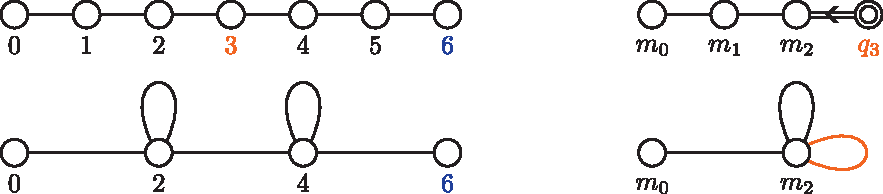
\includegraphics{SU26SO36Dynkin.pdf}
\caption{\label{SUSOsix} The upper left diagram is the principle graph of $SU(2)_6$, and the 
lower left diagram is the principle graph for $SO(3)_6$. 
On the right we give the principle graphs of the condensed theories $SU(2)_6/\psi$ (top right) and 
$SO(3)_6/\psi$ (bottom right), both with the identification $\psi=6$. 
The naming convention of the condensed theories has been inherited from the parent theories, 
along with an $m$ or $q$ denoting whether the particle is m-type or q-type.
Black links denote even fusion channels, and the red link connecting $m_2$ to itself 
denotes an odd fusion channel in accordance with the rule $m_2\tp m_2 \cong m_0 \oplus \cc^{1|1}m_2$. 
}
\end{figure}
The particles $0,2,4,$ and $6$ form a closed sub-category of $SU(2)_6$. 
The principle graph of this theory is shown in the bottom left of Fig.~\ref{SUSOsix}. 
%The principle graph of this theory is found by removing the particles $1,3,5$ in the principle graph of $SU(2)_6$, shown in the bottom left of Fig.~\ref{SUSOsix}. 
This is the subcategory known as $SO(3)_6$, it is a braided theory, with braiding and 
fusion inherited from $SU(2)_6$, however, it is not modular.
The $6$ particle braids trivially within this subcategory, and is therefore transparent, 
which breaks the modularity.

We now perform fermion condensation in $SU(2)_6$ and $SO(3)_6$ to obtain two super pivotal 
categories $SU(2)_6/\psi$ and $SO(3)_6/\psi$. 
Since $\psi$ is not transparent in $SU(2)_6$, we must perform the back-wall condensation 
process described earlier. 
However, since $\psi$ {\it is} transparent in $SO(3)_6$, condensation of $\psi$ is possible 
without employing a back-wall (although a spin structure is still needed). 
The principle graphs of the condensed theories are shown on the right of Fig.~\ref{SUSOsix}.
The simple objects of the two theories are given as follows:
\begin{align}
\xymatrix @!0 @M=1mm @C=10mm {
SU(2)_6/\psi:&&m_0 & m_1 & m_2 & q_3 \\
SO(3)_6/ \psi:&&m_0 && m_2& 
}
\end{align}
The particles have a natural grading given by (\ref{grading}) with the even set given by 
$I_0 = \{ m_0, m_2 \}$ and the odd set given by $I_1 = \{m_1, q_3\}$, with $I_a \tp I_b = I_{a+b \;  \text{mod} \; 2}$.
The closed sub-fusion algebra given by $I_0$ contains all of the objects in $SO(3)_6/\psi$, 
which occurs since $\psi$ is transparent in $SO(3)_6$. 
Note that there are no q-type objects in $SO(3)_6/\psi$. 

The non-trivial fusion rules of $SU(2)_6/\psi$ are given in Table \ref{SU2six_psi_fusion}.
%\dave{Should put these in our standard form.}
%\dave{Put into our standard form, should double check though.}
%\dave{We should make this a table and not an equation, I'll do that soon.}
\begin{table} 
\begin{align}
\xymatrix{
\text{
{\tabulinesep=1.2mm
\begin{tabu}{ c | c c  c c |c  c   }
$I_0 \tp I_0$&$m_0$ &$m_2$&$\quad\quad$&
$I_0 \tp I_1$&$m_1 $& $q_3$\\  
\cline{1-3}\cline{5-7}$m_0$&$m_0$ & $m_2$ &&
$m_0$& $m_1 $& $q_3$\\   
$m_2$ & $m_2$ & $m_0 \oplus \mathbb{C}^{1|1}m_2$&&
$m_2$ &$ m_1\oplus q_3 $ & $\mathbb{C}^{1|1} m_1 \oplus q_3$\\
\multicolumn{1}{r}{}&& &&\multicolumn{1}{r}{}&&\\
$I_1 \tp I_0$&$m_0 $& $m_2$ &&
$I_1 \tp I_1$ &$m_1 $& $q_3$\\  
\cline{1-3}\cline{5-7} $m_1$& $m_1 $& $m_1\oplus q_3$ &&
$m_1$ &$m_0 \oplus m_2$&$ \mathbb{C}^{1|1} m_2$ \\
$q_3$ &$ q_3  $ & $\mathbb{C}^{1|1} m_1 \oplus q_3$ &&
$q_3$ &$\mathbb{C}^{1|1} m_2 $&$ \mathbb{C}^{1|1}m_0 \oplus \mathbb{C}^{1|1}m_2$\\
\end{tabu}
}}
}
\end{align}
\caption{Fusion rules for $SU(2)_6/\psi$
\label{SU2six_psi_fusion}}
\end{table}

We note two features of these examples which were not present in our earlier $C_2$ example:
\begin{itemize}
\item Even though $m_2$ is an m-type particle, $\mathbb{C}^{1|1}m_2$ 
appears in the tensor product of $m_2$ with itself.
So $SO(3)_6/\psi$ provides us with an example of a theory which has 
no q-type objects, but which is still fermionic in the sense that its fusion spaces contain both even and odd elements. 
%\dave{Should we say  `...its fusion spaces contain both even and odd elements.'. 
%Is a ``non-intrinsically" fermionic theory one where the parity of a fusion space  $V^{abc \cdots}$ is fixed by $abc \cdots$?
%}
%\kw{``intrinsically" was not my word choice; dropped it.  I think we are not making a very precise observation here, which is fine.}
\item The q-type particle $q_3$ appears in the tensor product of two m-type 
particles, namely $m_2 \tp m_1$. 
Thus our classification of simple objects as m- or q-type should not be thought of as a $\zz/2$ grading, since the types of 
$a$ and $b$ in no way constrain the possible types of the simple objects appearing in $a\tp b$.
(In the next section we will also see an example of two q-type particles fusing to another q-type particle.)
\end{itemize}


%There are two peculiarities that these examples highlight nicely. 
%First, we observe that $m_2$ is an m-type particle, despite the fact that $\mathbb{C}^{1|1}m_2$ 
%appears in the tensor product of $m_2$ with itself.
%Since $m_2\in SO(3)_6/\psi$, $SO(3)_6/\psi$ provides us with an example of a theory which has 
%no q-type objects, but which is still intrinsically ``fermionic'', in the sense that its fusion spaces contain odd elements. 
%
%Second, we note that the q-type particle $q_3$ appears in the tensor product of two m-type 
%particles, namely $m_2 \tp m_1$. 
%Therefore, it is perfectly consistent to have two m-type particles fuse to a q-type particle, meaning 
%that the fusion rules do not respect the $\zt$ 
%decomposition of objects according to their type, 
%unlike the finite-group-based models in Refs \cite{bhardwaj2016,kapustin2017} where the type of objects is determined 
%by a homomorphism $\sigma : \mcc \ra \zt$. 
%%\ethan{$\mcc$ is always a finite group for these guys}
%%see e.g. page 36
%%\kw{Did Kapustin really assume this??  If so, presumably he was confusing the $\tp$ of simple super-algebras with the $\tp$ of anyons; same notation,
%%but very different things}
%%\ethan{Yes, he assumes that q-type guys are determined by a homomorphism $\pi : G \ra \zt$ (he only considers $G$-graded Ising-type theories) which I think is actually a natural guess from a physical point of view. Should quadruple check, though. Relevant stuff to look for is the Ising pull-backs in the big paper and the $\pi_1$ in the paper with just Gaiotto.}
%%\dave{Lets double check this before removing the comments.}
%\dave{Ethan, did you the quadruple check of this fact?
%I haven't read the relevant parts of those papers yet.}
%\ethan{I've checked it a few times, yeah. Look at page 36 of the fermionic state-sum 
%Kapustin-Gaiotto-Bsomeone paper, I think. We can remove the reference though, if it seems too confrontational} 
%Interestingly, $q_3$ appears in $m_2 \tp m_1$ with coefficient $\mathbb{C}^{1|0}$, despite the fact that $V^{m_2 m_1}_{q_3} \cong \mathbb{C}^{1|1}$.

The $F$-symbols of the condensed theories can be deduced from those of the parent theories, so we will not list them here.
We now compute the minimal idempotents of the tube algebra in the condensed theories.


%%%%%%%%%%%%%%%%%%%%%%%%%%%
\subsection{Primitive idempotents of $SU(2)_6/\psi$}
\label{SU2psiIdempotents}
%%%%%%%%%%%%%%%%%%%%%%%%%%%

The primitive idempotents of the tube category of $SU(2)_6/\psi$ can be computed directly 
using the techniques of Section \ref{more_on_tubes}. 
They are given by
\begin{align}
E(a,b) = \TubeIdempotentTwoStrandab_{J}, \quad \quad  (a,b) \in \sob(SU(2)_6) \times \sob(SU(2)_6/\psi),
\end{align}
where as before we require that $s(J) = (-1)^{\nu_b}$.
It will be useful to recast these idempotents in a form 
that can easily used to compute the idempotents for $SO(3)_6$. 
We first define
\begin{align}
\widetilde{E}(a,b,\text{cl}(r)) \; = \; \BasisForIdempotents
\end{align}
and for $x = \unit$ or $x = \psi$ we define the $\omega_x$ loop 
%$\omega$ loop $\omega_x$ by 
%\dave{Maybe this: `we define the $\omega_x$ loop'}
\begin{align}
 \omega_x = \frac{d_x}{\mathcal{D}_{\mcc/\psi}^2} \sum_{r\in \sob(\mcc/\psi)} \frac{d_r }{ \dim\End(r)} \left( \frac{S_{xr}}{S_{\unit r}} \right)   \text{cl}(r).
\end{align}
The $S$-matrix above is that of the parent theory, and the labels are trivial lifts from $\mcc/\psi$.
When $x = \unit$, $ \frac{S_{x r}}{S_{\unit r}}=1$ this is just the standard $\omega$ loop, 
when $x =\psi$, $ \frac{S_{x r}}{S_{\unit r}}=(-1)^{\nu_r}$ and $\omega_\psi$ is a projector onto the $\psi$ strand.
The factor $\mcd_{\mcc/\psi}^2 = \sum_{x \in \mcc/\psi} d_x^2 / \dim \End(x)$ is the total quantum dimension of 
the condensed theory in the sense of \eqref{total_qdim_defn}. 
The minimal idempotents given by $E(a,b)$ in \eqref{FunctorCxCtoTubeC}
can be re-written as
\begin{align}
E(a\tp x, b) \cong \widetilde{E}(a,b, \omega_x),
\end{align}
with $a,b \in \mcc/\psi$ and $x =\unit, \psi$.
The isomorphism relating the two idempotents is an odd isomorphism if $x = \psi$.
Notice that running over all all pairs $a,b \in \mcc/\psi$ and $x = \unit$ or $\psi$ runs over all possible $E(a,b)$.
Additionally if $a \tp \psi \cong a$ then $\widetilde{E}(a,b, \omega_\unit)$ and $\widetilde{E}(a,b, \omega_\psi)$ are equivalent. 
This presentation of the idempotents is more symmetric than those discussed in Section \ref{more_on_tubes}.

We now write these idempotents so that they have a single strand at the boundary rather than two.
We use the fermionic analogue of \eqref{TwoStrandToOneStrand}
%and replace $\omega$ by $\omega_x$,
%\begin{align}
%g(a,b,\omega_x,c,j) = \gxyajf  \quad \quad \quad h(a,b,\omega_x,c,i) = \hxyaif
%\end{align}
to write down the single strand idempotents
\begin{align}
\label{OneStrandIdempotent}
\tilde{e}_{ab}(\omega_x,c,j) \; = \; \OneStrandIdempotentMTCpsi.
%g(a,b,\omega_x,c,j)  \cdot h(a,b,\omega_x,c,j) 
\end{align}
These idempotents are essentially the same as the ones described earlier in \eqref{idempotent_one_strand}. 
The particular representative of the isomorphism class is given by choosing $c \in a\tp b$, and appropriatey normalized vectors $\mu_j \in V^{ab}_c(\mcc/\psi)$, and $\nu_j \in V^{c}_{ab}(\mcc/\psi)$.
We will denote the parity of $\mu_j \in V^{ab}_c(\mcc/\psi)$ by $\sigma_j=1$ $(\sigma_j = -1)$ if the chosen basis vector $\mu_j$ in the fusion space $V^{ab}_c(\mcc/\psi)$ is even (odd).
The twists of the idempotents are given by 
\begin{align} 
\label{CmodPsiTwistsModular}
T\cdot \tilde{e}(a,b,\omega_x,c,j)  =\left[  \frac{\theta_a}{\theta_b} (-1)^{x (\nu_a + \nu_b)}(-s(J))^{(1-\sigma_j)/2}  \right ] \tilde{e}(a,b,\omega_x,c,j)
\end{align}
We will write $\tilde{e}(a,b,\omega_x,c,j)$ as $m_{ab}(\omega_x,c,j)$ 
if the idempotent is m-type and $q_{ab}(\omega_x,c,j)$ if the idempotent is q-type.
For $SU(2)_6/\psi$ we list a complete set of representatives of minimal idempotents.
We find 14 m-type idempotents for the bounding spin structure, 
and 14 idempotents for the non-bounding spin structure, 7 are m-type and 7 are q-type. 
Explicitly, the idempotents and corresponding twists are listed in tables \ref{bounding_SU26} and \ref{nonbounding_SU26}.
Note that if $a$ is q-type, then $\tilde{e}(a,b,\omega_\unit,j)$ is isomorphic to $\tilde{e}(a,b,\omega_\psi,j)$ and so we only list one of them.
We now turn our attention to the $SO(3)_6$ theory. 
\begin{table}
\begin{center}
\begin{align}
\nonumber
\xymatrix @M=0mm @R=5mm @C=5mm {
&\text{
\begin{tabu}{ c | c }
type& $\quad$twist $\quad$ \\ \hline
$m_{00}(\omega_0,c,j)$ &$1$ \\
$m_{10}(\omega_0,c,j)$ &$e^{3 i \pi /16}$ \\
$m_{20}(\omega_0,c,j)$ &$i$ \\
\end{tabu}
}
&
\text{
\begin{tabu}{ c | c }
type& $\quad$twist $\quad$  \\ \hline
$m_{00}(\omega_\psi,c,j)$ &$1$ \\
$m_{10}(\omega_\psi,c,j)$ &$-e^{3 i \pi/16}$ \\
$m_{20}(\omega_\psi,c,j)$ &$i$ \\
\end{tabu}
}
&
\text{
\begin{tabu}{ c | c }
type& twist $\times \; \sigma_j$ \\ \hline
$m_{30}(\omega_0,c,j)$ &$ e^{15i \pi /16}$ \\
$m_{32}(\omega_0,c,j)$ &$-ie^{15i \pi /16}$ \\
\end{tabu}
}
\\
&\text{
\begin{tabu}{ c | c }
type& twist $\times \; \sigma_j $ \\ \hline
$m_{02}(\omega_0,c,j)$ &$-i $ \\
$m_{12}(\omega_0,c,j)$ &$-i e^{3 i \pi/16}$ \\
$m_{22}(\omega_0,c,j)$ &$1$ \\
\end{tabu}
}
&
\text{
\begin{tabu}{ c | c }
type&twist $\times \; \sigma_j $ \\ \hline
$m_{02}(\omega_\psi,c,j)$ &$-i$ \\
$m_{12}(\omega_\psi,c,j)$ &$ie^{3 i \pi /16}$ \\
$m_{22}(\omega_\psi,c,j)$ &$1$ \\
\end{tabu}
}&}
\end{align}
\caption{ Bounding idempotents for $SU(2)_6/\psi$.
Where $c \in a \tp b$ and $j$ labels the choice of in the fusion space $V^{ab}_c (\mcc/\psi)$.
Some of these labels are determined, 
e.g., $m_{00}(\omega_0,c,j)$ can be simplified to $m_{00}(\omega_0,m_0,0)$.
}
\label{bounding_SU26}
\end{center}
\end{table}

\begin{table}
\begin{center}
\begin{align}
\nonumber
\xymatrix @M=0mm @R=5mm @C=5mm  {
&\text{
\begin{tabu}{ c | c }
type&$\quad  $ twist $\quad \;$ \\ \hline
$m_{01}(\omega_0,c,j)$ &$-e^{-3i\pi/16}$ \\
$m_{11}(\omega_0,c,j)$ &$1$ \\
$m_{21}(\omega_0,c,j)$ &$-i e^{-3i \pi /16}$ \\
\end{tabu}
}
&
\text{
\begin{tabu}{ c | c }
type& $\quad  $ twist $\quad \;$ \\ \hline
$m_{01}(\omega_\psi,c,j)$ &$-e^{-3 i \pi /16}$ \\
$m_{11}(\omega_\psi,c,j)$ &$1$ \\
$m_{21}(\omega_\psi,c,j)$ &$-i e^{-3 i \pi /16}$ \\
\end{tabu}
}
&
\text{
\begin{tabu}{ c | c }
type& twist \\ \hline
$m_{31}(\omega_0,c,j)$ &$e^{3 i \pi /4}$ \\
$q_{33}(\omega_0,c,j)$ &$1$ \\
\end{tabu}
}
\\
&\text{
\begin{tabu}{ c | c }
type& twist \\ \hline
$q_{03}(\omega_0,c,j)$ &$-e^{-15 i \pi /16}$ \\
$q_{13}(\omega_0,c,j)$ &$e^{- 3 i \pi /4}$ \\
$q_{23}(\omega_0,c,j)$ &$-i e^{-15 i \pi /16}$ \\
\end{tabu}
}
&
\text{
\begin{tabu}{ c | c }
type& twist \\ \hline
$q_{03}(\omega_\psi,c,j)$ &$-e^{-15 i \pi /16}$ \\
$q_{13}(\omega_\psi,c,j)$ &$e^{- 3 i \pi /4}$ \\
$q_{23}(\omega_\psi,c,j)$ &$- i e^{- 15i \pi /16}$ \\
\end{tabu}
}&
}
\end{align}
\caption{Non-Bounding idempotents for $SU(2)_6/\psi$
}
\label{nonbounding_SU26}
\end{center}
\end{table}




\begin{comment}
%%%%%%%%%%%%%%%%%%%%%%%%%%%%%%
\subsection{Primitive idempotents of $SU(2)_6/\psi$}
%%%%%%%%%%%%%%%%%%%%%%%%%%%%%%
\dave{Thinking about how to improve this discussion and tie it in with Section 5. 
Obviously in progress, need to check some things.}
\begin{enumerate} 
\item list idempotents of $SU(2)_6 /\psi$ via $E(a,b)$, $a \in \mcc$, $b \in \mcc/\psi$
\item Define the isomorphic set of idempotents $\widetilde{E}(a,b,x) \cong E(a\tp x,b)$. $\widetilde{E}(a,b,x)$ is the same as $E(a,b)$ but we replace the $\omega$ loop with an $\omega_x$ loop.
The complete set of idempotents is given by $\widetilde{E}(a,b,x)$, $a,b\in \mcc/\psi$ and $x =\unit, \psi$. 
\item observe that if $a , b \in SO(3)_6/\psi$ then $E(a,b, \unit \oplus \psi)$ is a minimal idempotent for $\tube^B(SO(3)_6/\psi)$
\item Next do the case where $a \tp b \in SO(3)_6/\psi$.
Find a tensor functor from $\widetilde{\tube}(SU(2)_6/\psi)$ to $\tube(SO(3)_6/\psi)$.
Idea is to look at $\tube(SU(2)_6/\psi)$ but constrain the allowed morphisms so that they have a nice inclusion into $\tube(SO(3)_6/\psi)$.
(weight out this option with the 1-strand idempotent option, or mention both)
\end{enumerate} 


%\dave{Dropped some redundant things that were already in Section \ref{more_on_tubes}
%feel free to un-drop them.}

The primitive idempotents of the tube category of $SU(2)_6/\psi$ can be computed directly 
from the primitive idempotents of the parent theory $SU(2)_6$ by condensing a fermion
in $\tube(SU(2)_6)$, as discussed in Section \ref{more_on_tubes}. 
%The primitive idempotents of the tube category of $SU(2)_6/\psi$ can be computed directly 
%from the primitive idempotents of the parent theory $SU(2)_6$ by ``condensing" the fermions off of the elements in $\tube(SU(2)_6)$. 
%This procedure always produces minimal idempotents in $\tube(SU(2)_6/\psi)$, 
%although the process is rarely straightforward: condensing $\psi$ in $\tube(SU(2)_6)$ 
%may send some of the idempotents to zero, enlarge the isomorphism classes or identify some idempotents with others, etc.
%For brevity's sake, we will only present the results of the calculations in what follows. 
For the example at hand, we find it convenient to adopt a specific presentation of the idempotents 
which is essentially the same as the one described earlier in \eqref{idempotent_one_strand}. 
For any MTC, we can write the idempotents in $\mcc/\psi$ as 
%\ethan{minor quibble: in this figure and in some in the next two subsections, some lines are drawn in orange---any stylistic reason why?}
%\dave{I had no reason. I can change it to black.}
\dave{Will change twist when we decide how we are going to talk about them, both here and below.}
\begin{align}
\xymatrix{
f_{ab}^x 
=\sqrt{\frac{d_a d_b}{d_c}} \underset{\quad \quad c \; \in \; a \tp b}{\IdempBraid{a}{b}{}{\omega_x}{J}}
&
\text{
{\tabulinesep=1.2mm
\begin{tabu}{ r c }
%consistency constraint: & $ (-1)^{s(J) + \nu_b}=1$ \\ 
consistency constraint: & $ s(J)(-1)^{\nu_b}=1$ \\ 
%topological twist:& $\frac{\theta_a}{\theta_b} (-1)^{(s(J)+1)p_{ab}^c + x(\nu_a + \nu_b)}$ \\
topological twist:& $\frac{\theta_a}{\theta_b} (-s(J))^{p_{ab}^c}(-1)^{x(\nu_a + \nu_b)}$
%isomorphism class: & $c \in a \tp b$
\end{tabu}
}}
}
\end{align} 
\kw{I don't understand what's meant by ``isomorphism class: $c \in a \tp b$"}
\dave{dropped it. }
\dave{I think $f_{ab}^c$ should actually be $f_{ab}^x$ denoting whether $x =0$ or $x =\psi$.}
where as before $s(J) = 1$ ($s(J)=-1)$ if $J=B$ ($J=N$) and $x=0$ denotes the presence of an $\omega$ loop 
in the annulus on the left while $x=1$ corresponds to the presence of an $\omega_\psi$ loop in the annulus, 
where $\omega_x$ is defined by 
\begin{align}
 \omega_x = \frac{1}{\mathcal{D}_{\mcc/\psi}^2} \sum_{r\in \sob(\mcc/\psi)} \frac{d_r }{ \dim\End(r)} (-1)^{x \nu_r}   \text{cl}(r),
\end{align}
\dave{dropped the factor of $2$ above to be consistent with the following.}
\kw{which factor of 2 was dropped?}
\dave{There was a factor of $2$ in the numerator at some point.
I think at one point I just had $\mcd^2$ in the denominator and it was unlclear if that was for the parent theory or the condensed one and lead to an inconsistency once the following sentence was added.
}
and $\mcd_{\mcc/\psi}^2 = \sum_{x \in \mcc/\psi} d_x^2 / \dim \End(x)$ is the total quantum dimension of 
the condensed theory in the sense of \eqref{total_qdim_defn}. 
The particular representative of the isomorphism class is given by choosing $c \in a\tp b$, and a vector from $V^{ab}_c(\mcc/\psi)$.
Finally, we have defined $p_{ab}^c$ in the twist of the idempotent by $p_{ab}^c=0$ ($p^c_{ab}=1$) 
if the chosen basis vector in the fusion space $V^{ab}_c(\mcc/\psi)$ is even (odd).
Note that in the language of Section~\ref{double_fermionic_quotient} the $f_{ab}^x$ are isomorphic to $E(a \tp x, b)$.
In what follows, we will write $f^x_{ab}$ as $m^x_{ab}$ 
\kw{Up unitl now we have been using lower case letters for idempotents, so maybe this should
be changed to  $m^c_{ab}$?}
\dave{Yes, agreed.}
if the idempotent is m-type (i.e. not invariant under fusion with $\psi$)
and $f^x_{ab}$ as $q^x_{ab}$ if the idempotent is q-type (i.e. has an odd endomorphism / is invariant under fusion with $\psi$).
%Note that by our previous discussion in Section \ref{more_on_tubes}, if $b$ is a q-type object 
%then the idempotent $f^x_{ab}$ must be associated with a non-bounding spin structure. \dave{I don't think this needs to be said here.}
\kw{How does this paragraph line up with the current version of Section 5?}


In the case of $SU(2)_6$ we find 14 m-type idempotents for the bounding spin structure, 
and $7$ m-type as well as $7$ q-type idempotents for the non-bounding spin structure. 
\dave{Need to check this again carefully and do sum of squares..}
\dave{Should we remove the twist stuff?}
\begin{align}
&\text{
\begin{tabu}{ c | c }
type& twist \\ \hline
$m_{00}^0$ &$1$ \\
$m_{10}^0$ &$e^{3 i \pi /16}$ \\
$m_{20}^0$ &$i$ \\
\end{tabu}
}
\quad \quad
\text{
\begin{tabu}{ c | c }
type& twist  \\ \hline
$m_{00}^\psi$ &$1$ \\
$m_{10}^\psi$ &$-e^{3 i \pi/16}$ \\
$m_{20}^\psi$ &$i$ \\
\end{tabu}
}
\quad \quad
\text{
\begin{tabu}{ c | c }
type& twist $\times \; (-1)^{p_{ab}^c} $ \\ \hline
$m_{30}^0$ &$ e^{15i \pi /16}$ \\
$m_{32}^0$ &$-ie^{15i \pi /16}$ \\
\end{tabu}
}
\\
&\text{
\begin{tabu}{ c | c }
type& twist $\times \; (-1)^{p_{ab}^c} $ \\ \hline
$m_{02}^0$ &$-i $ \\
$m_{12}^0$ &$-i e^{3 i \pi/16}$ \\
$m_{22}^0$ &$1$ \\
\end{tabu}
}
\quad \quad
\text{
\begin{tabu}{ c | c }
type&twist $\times \; (-1)^{p_{ab}^c} $ \\ \hline
$m_{02}^\psi$ &$-i$ \\
$m_{12}^\psi$ &$ie^{3 i \pi /16}$ \\
$m_{22}^\psi$ &$1$ \\
\end{tabu}
}
\end{align}
while in the non-bounding spin structure sector we find
\begin{align}
&\text{
\begin{tabu}{ c | c }
type& twist \\ \hline
$m_{01}^0$ &$-e^{-3i\pi/16}$ \\
$m_{11}^0$ &$1$ \\
$m_{21}^0$ &$-i e^{-3i \pi /16}$ \\
\end{tabu}
}
\quad \quad
\text{
\begin{tabu}{ c | c }
type& twist \\ \hline
$m_{01}^\psi$ &$-e^{-3 i \pi /16}$ \\
$m_{11}^\psi$ &$1$ \\
$m_{21}^\psi$ &$-i e^{-3 i \pi /16}$ \\
\end{tabu}
}
\quad \quad
\text{
\begin{tabu}{ c | c }
type& twist \\ \hline
$m_{31}^0$ &$e^{3 i \pi /4}$ \\
$q_{33}^0$ &$1$ \\
\end{tabu}
}
\\
&\text{
\begin{tabu}{ c | c }
type& twist \\ \hline
$q_{03}^0$ &$-e^{-15 i \pi /16}$ \\
$q_{13}^0$ &$e^{- 3 i \pi /4}$ \\
$q_{23}^0$ &$-i e^{-15 i \pi /16}$ \\
\end{tabu}
}
\quad \quad
\text{
\begin{tabu}{ c | c }
type& twist \\ \hline
$q_{03}^\psi$ &$-e^{-15 i \pi /16}$ \\
$q_{13}^\psi$ &$e^{- 3 i \pi /4}$ \\
$q_{23}^\psi$ &$- i e^{- 15i \pi /16}$ \\
\end{tabu}
}
\end{align}
We now turn our attention to the $SO(3)_6$ theory. 
\end{comment}


%%%%%%%%%%%%%%%%%%%%%%%%%%%%%%
\subsection{Primitive idempotents of $SO(3)_6/\psi$}
%%%%%%%%%%%%%%%%%%%%%%%%%%%%%%

Finding the idempotents in the $SO(3)_6/\psi$ theory is more difficult, since the parent theory $SO(3)_6$ isn't modular.
%\dave{drop next sentence?}
%However, the sole cause of its non-modularity is the transparent fermion $\psi$, 
%and it can be made modular by performing a ``modular extension'' and introducing defects 
%which braid non-trivially with $\psi$, see \cite{bruillard2017} for more details.
However since $SO(3)_6$ is obtained from $SU(2)_6$ by discarding the elements in $SU(2)_6$ 
that braid nontrivially with $\psi$, $SU(2)_6$ is a modular extension of $SO(3)_6$ (in fact, it is the minimal modular extension). 
This fact will allow us to compute the idempotents in the $SO(3)_6/\psi$ theory using our knowledge of the $SU(2)_6$ theory. 

Applying \eqref{OneStrandIdempotent} directly to $SO(3)_6$ will not yield a complete set of minimal idempotents due to the lack of modularity. 
Instead we use  \eqref{OneStrandIdempotent} by taking pairs of simple objects $(a,b)$ from $SU(2)_6/\psi \times SU(2)_6/\psi$ whose tensor product is always in $SO(3)_6/\psi$.
Additionally, within this subset we need to take an appropriate linear combination of the $SU(2)_6/\psi$ idempotents so that the resulting annulus only has strands labeled by objects in $SO(3)_6/\psi$.
This linear combination is given by taking $\tilde{e}_{ab}(\omega_\unit, c,j)+\tilde{e}_{ab}(\omega_\psi, c,j)$ which results in the minimal idempotent
%\dave{need to fix $\tilde{(}$}
\begin{align}
\widetilde{e}_{ab}( \omega_\unit + \omega_\psi,c,j) \in \tube(SO(3))_6).
\end{align}
where the labels $(a,b) \in I_0/\psi \times I_0/\psi \cup I_1/\psi \times I_1/\psi$.
One can show that the procedure creates a complete set of minimal idempotents by direct calculation. 
The bounding idempotents are found when $(a,b) \in I_0/\psi \times I_0/\psi$, 
these are the minimal idempotents found from a naive application of \eqref{OneStrandIdempotent}. 
The non-bounding idempotents are given by $(a,b) \in I_1/\psi \times I_1/\psi$



%However, by taking linear combinations of an appropriate subset of the $SU(2)_6$ idempotents we will find the $SO(3)_6$ idemopotents. 
%The relavent subset and linear combinations are given by 
%\begin{align}
 %\widetilde{e}_{ab}( \omega_\unit + \omega_\psi,c,j) \quad \quad (a,b) \in I_0 \times I_0 \cup I_1 \times I_1.
%\end{align}
%The restriction on the labels $(a,b)$ is so that $a \tp b \in SO(3)_6$. 
%The linear combination $\omega_\unit + \omega_\psi$ is taken so that the omega loop for $SO(3)_6$.
\begin{comment}
\dave{Older stuff.}
As before, each isomorphism class of idempotents can be written as:
\begin{align}
\xymatrix{
\sqrt{\frac{d_a d_b}{d_c}} \underset{\quad \quad c \; \in \; a \tp b}{\IdempBraid{a}{b}{}{\omega}{J}}
&
a,b \in \sob(SU(2)_6/\psi) \quad \text{such that} \quad a \tp b \in \sob(SO(3)_6/\psi) 
}
\label{SO3idempotent}
\end{align}
where $J$ denotes the spin structure of the annulus, 
and we are using the normalization conventions of \cite{Bonderson2007}.
The $\omega$ loop is for $SO(3)_6/\psi$. 
If we take $a,b \in \sob(SO(3)_6/\psi)$ (rather than in $\sob(SU(2)_6/\psi)$, then we will miss several idempotents. 
The key observation is that we can take pairs of simple objects $(a,b)$ from $SU(2)_6/\psi$ whose fusion product is always in $SO(3)_6/\psi$.
Hence the idempotents of $\tube(SO(3)_6/\psi)$ are just a restriction of the idempotents of $\tube(SU(2)_6/\psi)$. 
One can show that the procedure creates orthogonal idempotents by direct calculation. 
Additionally, the tube resulting from fusing the strands in (\ref{SO3idempotent}) 
into the annulus only contains linear combinations of tubes in the annular category of $SO(3)_6/\psi$.
\end{comment} 


We now write down the primitive idempotents of $SO(3)_6/\psi$ and their twists using the same notation as in section \ref{SU2psiIdempotents}. 
In the bounding sector $J = B$, we have $4$ m-type idempotents, given by
\begin{align}
\xymatrix{
%\underset{\quad \quad c \; \in \; a \tp b}{\IdempBraid{a}{b}{}{\omega}{B}}
%&
\text{
{{\tabulinesep=1.2mm
\begin{tabu}{ c c  }
type& twist \\ \hline
$m_{00}(\omega_\unit + \omega_\psi,0,0)$ &$1$ \\
$m_{02}(\omega_\unit + \omega_\psi,2,0)$ &$ -i $\\
$m_{20}(\omega_\unit + \omega_\psi,2,0)$ & $i$\\
$m_{22}(\omega_\unit + \omega_\psi,c,j)$ &$ \sigma_j $\\
\end{tabu}
}}}
} 
\end{align}
%where the column on the right displays the possible representatives of the isomorphism class, 
%whose coefficient denotes the possible parities of the fusion vertex on the idempotent. 
%For example, the idempotent $M_{22}$ has three possible representatives:
%one of them has boundary condition $m_0$, and the other two have boundary condition $m_2$. 
%The two fusion vertices of the idempotent with boundary condition $m_2$ can be either even or odd parity, 
%which is denoted by the coefficient $\cc^{1|1}$.
%Similarly, in the non-bounding sector we have 
%\dave{Comment on $Q_{13},Q_{31}$. There is only 1 idempotent.} \ethan{what does this mean?}
%\dave{There are two possible ways $1$ and $3$ can fuse to $m_2$, either evenly or oddly. 
%Above these led to two different idempotents, below they do not. 
%I added a paragraph on it, check it out and see if it clears things up.
%}
%\ethan{awesome!}
with $c \in m_2 \tp m_2$ and $j$ labeling a vector in the fusion space $V^{m_2 m_2}_c(\mcc/\psi)$.
Meanwhile the non-bounding idempotents are given by
\begin{align}
\xymatrix{
%\underset{\quad \quad c \; \in \; a \tp b}{\IdempBraid{a}{b}{}{\omega}{N}}
%&
\text{
{{\tabulinesep=1.2mm
\begin{tabu}{ c c }
type& twist \\ \hline
$m_{11}(\omega_\unit + \omega_\psi,c,j)$ &$1$ \\
$q_{13}(\omega_\unit + \omega_\psi,2,j)$ &$ e^{-3 i \pi/4} $\\
$q_{31}(\omega_\unit + \omega_\psi,2,j)$ & $e^{3 i \pi /4} $\\
$m_{33}(\omega_\unit + \omega_\psi,c,j)$ &$ 1 $\\
\end{tabu}
}}}
}
\end{align}
%\dave{Old table}.
%\begin{align}
%\xymatrix{
%\underset{\quad \quad c \; \in \; a \tp b}{\IdempBraid{a}{b}{}{\Omega_0}{N}}
%&
%\text{
%{{\tabulinesep=1.2mm
%\begin{tabu}{ c c | c }
%type& spin & isomorphism class \\ \hline
%$M_{11}$ &$1$&$\mathbb{C}^{1|0}m_0 \oplus \mathbb{C}^{1|0}m_2$ \\
%$Q_{13}$ &$ e^{-3 i \pi/4} $&$ \mathbb{C}^{1|1} m_2 $\\
%$Q_{31}$ & $e^{3 i \pi /4} $&$ \mathbb{C}^{1|1} m_2$\\
%$M_{33}$ &$ 1 $& $ \mathbb{C}^{1|0} m_0 \oplus  \mathbb{C}^{1|0} m_2$\\
%\end{tabu}
%}}}
%}
%\end{align}
%\dave{I need to convince myself of that last line again. Naively it could be $\mathbb{C}^{1|1} m_2$. But I think the oddly isomorphic idempotent is actually just the same idempotent.}
Similarly $c \in q_3 \tp q_3$ and $j$ labels a vector in $V^{q_3 q_3}_c(\mcc/\psi)$.
Here we've made use of the above observation that only $a \tp b$ need be in $SO(3)_6/\psi$, 
and hence the pairs $(a,b)$ in these idempotents are labeled by $m_1$ and $q_3$.
%Notice that for $Q_{13}$, $Q_{31}$, and $M_{33}$ the coefficient in front of $m_2$ is $\cc^{1|0}$, 
%and not $\cc^{1|1}$ as the fusion rules would indicate, see Table \ref{SU2six_psi_fusion}. 
%This is because $q_3$ is a q-type object in $SU(2)_6/\psi$, 
%and so it can freely ``absorb'' fermions (odd endomorphisms), which allows us to always ensure 
%that the vertices appearing in the idempotent have even parity. 
As the notation suggests $m_{33}$ is not q-type:
 to see this we note that if it were, then there would 
be an odd endomorphism of $\tube(SO(3)_6/\psi)$ with trivial boundary conditions (since $m_0 \in q_3 \tp q_3$).
That would require $SO(3)_6/\psi$ to contain a q-type simple object, 
but as explained in \eqref{noq-type} this is not possible since $\psi$ is transparent in $SO(3)_6$.
%But this isn't possible, since we would have an odd tube in $\tube(SO(3)_6/\psi)$ with trivial boundary conditions.
%This is only possible if $SO(3)_6/\psi$ has a particle with an odd endomorphism, 
%but as noted in \eqref{noq-type} this is not possible since $\psi$ is transparent in this theory.
One can explicitly construct an odd endomorphism for $q_{13}$ by putting a fermion on $q_3$ and fusing all strands into the annulus;
similarly for $q_{31}$. 
%\ethan{nice!}
%but as noted in \eqref{noq-type} transparency of $\psi$ exceludes this possibility.
%this is not possible since $\psi$ is transparent in this theory.
%One can explicitly construct an odd endomorphism for $Q_{13}$ by putting a fermion on $3$ and fusing all strands into the annulus. 
%Similarly for $Q_{31}$. 




%%%%%%%%%%%%%%%%%%%%%
\subsection{Modular transformations}
%%%%%%%%%%%%%%%%%%%%%

The modular transformations can be computed by direct calculation. 
%\dave{What are we going to say about spins?}
%\kw{I think we can leave the twist and T-matrix stuff more or less as is}
%\kw{Need to change ``spin" to ``twist" in this subsection}
%\dave{OK, I think I got all of them.}
We already have the twists (which are read off from the string-net labels of the idempotents), 
and the modular $T$-transformation can be obtained directly from the twists.
The modular $S$-transformation requires a little more work, 
and so we discuss this in a little more detail.

When gluing the idempotents along the boundary of the annulus we have to take linear combinations of 
idempotents in the same isomorphism class so that the glued up idempotent is invariant under local relations. 
Using the basis above, one finds
%\kw{in several places, including here, we write $\omega_0$ insead of plain $\omega$ as in Section 5.
%I think we should drop the subscript 0.}
\begin{align}
\tilde{e}_{ab}(\omega_\unit + \omega_\psi, c, j) \; \xrightarrow{\;\;  \text{cl}_Y \;\;  }\; \tilde{e}_{ab} \;=\;  \TorusBraidBasis{a}{b\;}{}{\omega}{X}{Y}
\end{align}
%\dave{I wrote it this way to avoid commenting on the sign $s(Y)$ that can appear if $\mu_j$ has odd parity.
%It seemed like it may cause more confusion than it's worth.
%We could add a footnote if we like.}
where $a$ and $b$ label the idempotent as before, $X$ denotes the spin structure of the idempotent which is fixed by $b$, $Y$ denotes the spin structure around the newly closed loop, 
and the $\omega$ loop is for the category $SO(3)_6/\psi$. 
Note that when $X$ is non-bounding, 
$a, b\in \{ m_1, q_3 \}$, which lies outside of $SO(3)_6/\psi$.
However, when the diagram is fused into the torus we find a torus string net labeled with objects only in $SO(3)_6/\psi$, as required.


In this graphical convention, the modular $S$-transformation acts as
\begin{align}
{ \TorusBraidBasis{a}{b\;}{}{\omega}{X}{Y}} \stackrel{S}{\longrightarrow} \sum_{r,w} S^{{XY \rightarrow YX}}_{(a,b),(r,w)} \;
{\TorusBraidBasis{r}{w}{}{\omega}{Y}{X} }\; .
\end{align}
The matrix elements can be computed explicitly using the $S$-matrix of $SU(2)_6$. 
\begin{comment}
\dave{This calculation is quite tedious.
It's almost quicker to just do it by brute force. 
I would say we remove the figure, and just tell the reader that the S-matrix can be found from direct calculation.
If we want to add more details about the calculation to version 2, we can do that.
}
In Fig.~\ref{SMatrixBFC} we have sketched one method to compute these matrix elements.
 \begin{figure}
  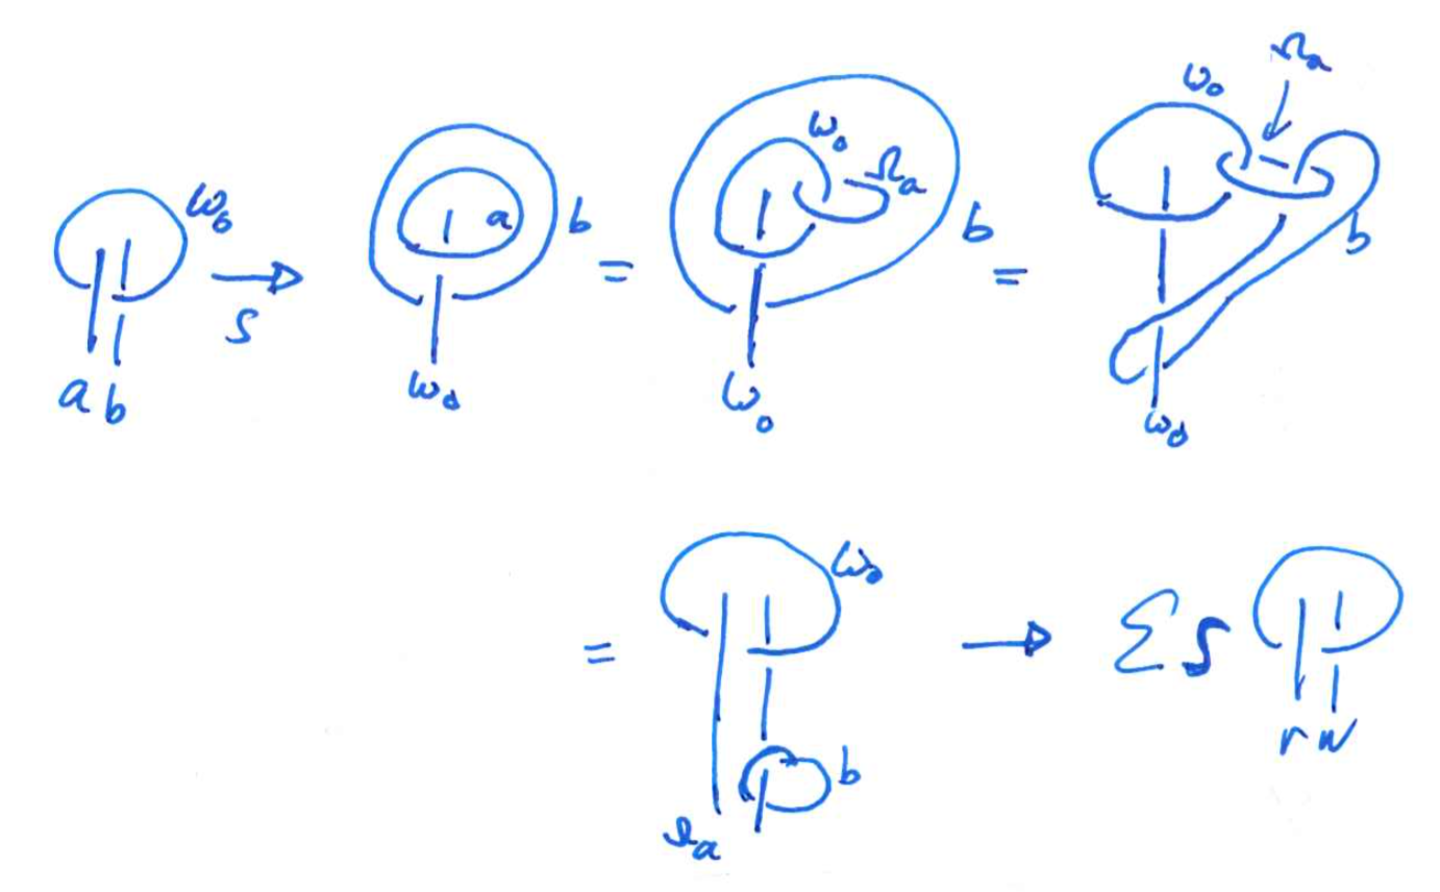
\includegraphics[scale=0.5]{SmatrixCalculationSketch.pdf}
 \caption{A caption describing the figure. \ethan{needs to be tex-ified eventually}
 \dave{Will do so soon.}
 \dave{I started doing this calculation and remembered that the above is just a cartoon, 
 the contents of which has been covered in the modular transformations part of Section 5.
 The actual calculation is a little more involved. 
 I think we should remove the Figure above, 
 and then either make the appropriate one, 
 or just bully the reader a bit and say `with some omega loop gymnastics one can find...'. 
}
\ethan{I like the last option, especially if we use the word `gymnastics'}
}
 \label{SMatrixBFC}
 \end{figure}
For the tori with one of the three spin structures possessing a bounding cycle (e.g.\ either $BB$, $BN$, or $NB$), we find 
\begin{align}
S^{{XY \rightarrow YX}}_{(a,b),(r,w)} = \frac{1}{(\sqrt{2})^{(n_a + n_b+n_r+n_w)}} \sin{\left( \frac{\pi(a+1)(r+1) }{8} \right)} \sin{\left(\frac{\pi(b+1)(w+1)}{8} \right)}
\end{align}
where $n_x = 0$ if $x = 0,1,2$ and $n_x = 1$ if $x = 3$ is an indicator distinguishing 
objects by their type (q or m).
The extra factors of $\sqrt{2}$ come from the fact that two of the idempotents in the non-bounding sector 
are q-type, and as such have endomorphism algebras of nontrivial dimension that affect how the $S$-
matrix is normalized.
\end{comment}
Explicitly, the $S$-matrix acts on each of the three bounding spin tori as 
\begin{align}
\left( \begin{matrix}
m_{00}\\
m_{02}\\
m_{20}\\
m_{22}\\
\end{matrix} \right)_{BB}
\xrightarrow{S^{BB \rightarrow BB}}
\frac{1}{2 \sqrt{2}} \left( \begin{matrix}
\frac{1}{d}&1&1&d \\
1& -\frac{1}{d} & d &-1 \\
1& d& -\frac{1}{d} & -1 \\
d & -1& -1& \frac{1}{d}\\
\end{matrix} \right)
\left( \begin{matrix}
m_{00}\\
m_{02}\\
m_{20}\\
m_{22}\\
\end{matrix} \right)_{BB}
\end{align}

\begin{align}
\left( \begin{matrix}
m_{11}\\
q_{13}\\
q_{31}\\
m_{33}\\
\end{matrix} \right)_{NB}
\xrightarrow{S^{NB \rightarrow BN}}
\frac{1}{2} \left( \begin{matrix}
1&1&1&1\\
1&-1&1&-1\\
1&1&-1&-1\\
1&-1&-1&1\\
\end{matrix} \right)
\left( \begin{matrix}
m_{00}\\
m_{02}\\
m_{20}\\
m_{22}\\
\end{matrix} \right)_{BN}
\end{align}

\begin{align}
\left( \begin{matrix}
m_{00}\\
m_{02}\\
m_{20}\\
m_{22}\\
\end{matrix} \right)_{BN}
\xrightarrow{S^{BN \rightarrow NB}}
\frac{1}{2} \left( \begin{matrix}
1&1&1&1\\
1&-1&1&-1\\
1&1&-1&-1\\
1&-1&-1&1\\
\end{matrix} \right)
\left( \begin{matrix}
m_{11}\\
q_{13}\\
q_{31}\\
m_{33}\\
\end{matrix} \right)_{NB}
\end{align}
As mentioned earlier, 
the Dehn twists follow directly from the twists computed above; 
see \eqref{CmodPsiTwistsModular}.
Again for the bounding spin tori we find
\begin{align}
\left( \begin{matrix}
m_{00}\\
m_{02}\\
m_{20}\\
m_{22}\\
\end{matrix} \right)_{BB}
\xrightarrow{T^{BB \rightarrow BN}}
\left( \begin{matrix}
1&&&\\
&-i&&\\
&&i&\\
&&&1\\
\end{matrix} \right)
\left( \begin{matrix}
m_{00}\\
m_{02}\\
m_{20}\\
m_{22}\\
\end{matrix} \right)_{BN}
\end{align}

\begin{align}
\left( \begin{matrix}
m_{11}\\
q_{13}\\
q_{31}\\
m_{33}\\
\end{matrix} \right)_{NB}
\xrightarrow{T^{NB \rightarrow NB}}
 \left( \begin{matrix}
 1&&&\\
&e^{-3 i \pi /4}&&\\
&&e^{3 i \pi /4}&\\
&&&1\\
\end{matrix} \right)
\left( \begin{matrix}
m_{11}\\
q_{13}\\
q_{31}\\
m_{33}\\
\end{matrix} \right)_{NB}
\end{align}

\begin{align}
\left( \begin{matrix}
m_{00}\\
m_{02}\\
m_{20}\\
m_{22}\\
\end{matrix} \right)_{BN}
\xrightarrow{T^{BN \rightarrow BB}}
\left( \begin{matrix}
1&&&\\
&-i&&\\
&&i&\\
&&&1\\
\end{matrix} \right)
\left( \begin{matrix}
m_{11}\\
q_{13}\\
q_{31}\\
m_{33}\\
\end{matrix} \right)_{BB}
\end{align}
One can verify that $(TS)^3 = \text{id}$, which holds since all three of the spin tori discussed above have 
 even fermion parity (recall that the more general identity is $(ST)^3 = (-1)^F$). 

The modular $S$ transformations on the torus with $NN$ spin structure are a little more tedious to calculate. 
%The m-type idempotents are always associated with spin tori whose ground states are fermion parity even, while the q-type idempotents are associated with ones with odd parity. 
A complete basis %for the ground-state
of net configurations on the $NN$ spin torus is given by
\begin{align}
\underbrace{
\xymatrix{
\TorusBraidBasisd{\scale{.6}{1}}{\scale{.6}{1}\;}{}{\omega}{N}{N}{\TorusBasisMTCNoLabel} \quad 
 \TorusBraidBasisd{\scale{.6}{3} }{\scale{.6}{3} \;}{}{\omega}{N}{N}{\TorusBasisMTCdd}
 \\}
 }_{\text{even}}
 \quad \quad 
\underbrace{
\xymatrix{ \TorusBraidBasisd{\scale{.6}{1}}{\scale{.6}{3}\;}{}{\omega}{N}{N}{\TorusBasisMTCdr} \quad
 \TorusBraidBasisd{\scale{.6}{3} }{\scale{.6}{1} \;}{}{\omega}{N}{N}{\TorusBasisMTCdl}
 \\}
 }_{\text{odd}}
\end{align}
%For this spin structure we find four states, which can be identified with two m-type and two q-type idempotents. 
On the non-bounding torus, m-type idempotents always close up into even parity states, 
while q-type idempotents close up into odd parity states.
The first two vectors have even parity and correspond to the closed up idempotents $m_{11}$ and $m_{33}$, 
while the second two have odd parity and correspond to the closed up idempotents $q_{13}$ and $q_{31}$.
After some calculation one finds that the $S$ and $T$ modular matrices act as 
\begin{align}
\xymatrix{
{\left( \begin{matrix}
m_{11}\\
m_{33}\\
\end{matrix} \right)_{NN}
\xrightarrow{S^{NN \rightarrow NN}}
 \left( \begin{matrix}
1&0\\
0&1\\
\end{matrix} \right)
\left( \begin{matrix}
m_{11}\\
m_{33}\\
\end{matrix} \right)_{NN}}
&
{
\left( \begin{matrix}
\stackrel{\bullet}{q}_{13}\\
\stackrel{\bullet}{q}_{31}\\
\end{matrix} \right)_{NN}
\xrightarrow{S^{NN \rightarrow NN}}
e^{- i \pi /4}\left( \begin{matrix}
1&0\\
0&i\\
\end{matrix} \right)
\left( \begin{matrix}
\stackrel{\bullet}{q}_{13}\\
\stackrel{\bullet}{q}_{31}\\
\end{matrix} \right)_{NN} 
}
\\
{
\left( \begin{matrix}
m_{11}\\
m_{33}\\
\end{matrix} \right)_{NN}
\xrightarrow{T^{NN \rightarrow NN}}
 \left( \begin{matrix}
1&0\\
0&1\\
\end{matrix} \right)
\left( \begin{matrix}
m_{11}\\
m_{33}\\
\end{matrix} \right)_{NN}
} & 
{
\left( \begin{matrix}
\stackrel{\bullet}{q}_{13}\\
\stackrel{\bullet}{q}_{31}\\
\end{matrix} \right)_{NN}
\xrightarrow{T^{NN \rightarrow NN}}
\left( \begin{matrix}
e^{-3i \pi /4}&0\\
0&e^{3 i \pi /4}\\
\end{matrix} \right)
\left( \begin{matrix}
\stackrel{\bullet}{q}_{13}\\
\stackrel{\bullet}{q}_{31}\\
\end{matrix} \right)_{NN}
}
} 
\end{align}
As required, the odd part of the $S$-matrix satisfies $S^4 = -\text{id}$ and $(TS)^3 = -\text{id}$, 
while the even part satisfies the usual $S^4 = \text{id}$ and $(TS)^3 = \text{id}$. 
%This provides us with an example of a theory in which the femion parity of the spin torus 
%%a ground state 
%is not uniquely determined from the ambient spin structure. 

